\documentclass[12pt, a4paper, twoside]{article}

%% Preamble
\usepackage{umatfgspanish}
\usepackage{blindtext}
\usepackage{listings}
\usepackage{subfig}
\graphicspath{ {./images/} }

\begin{document}

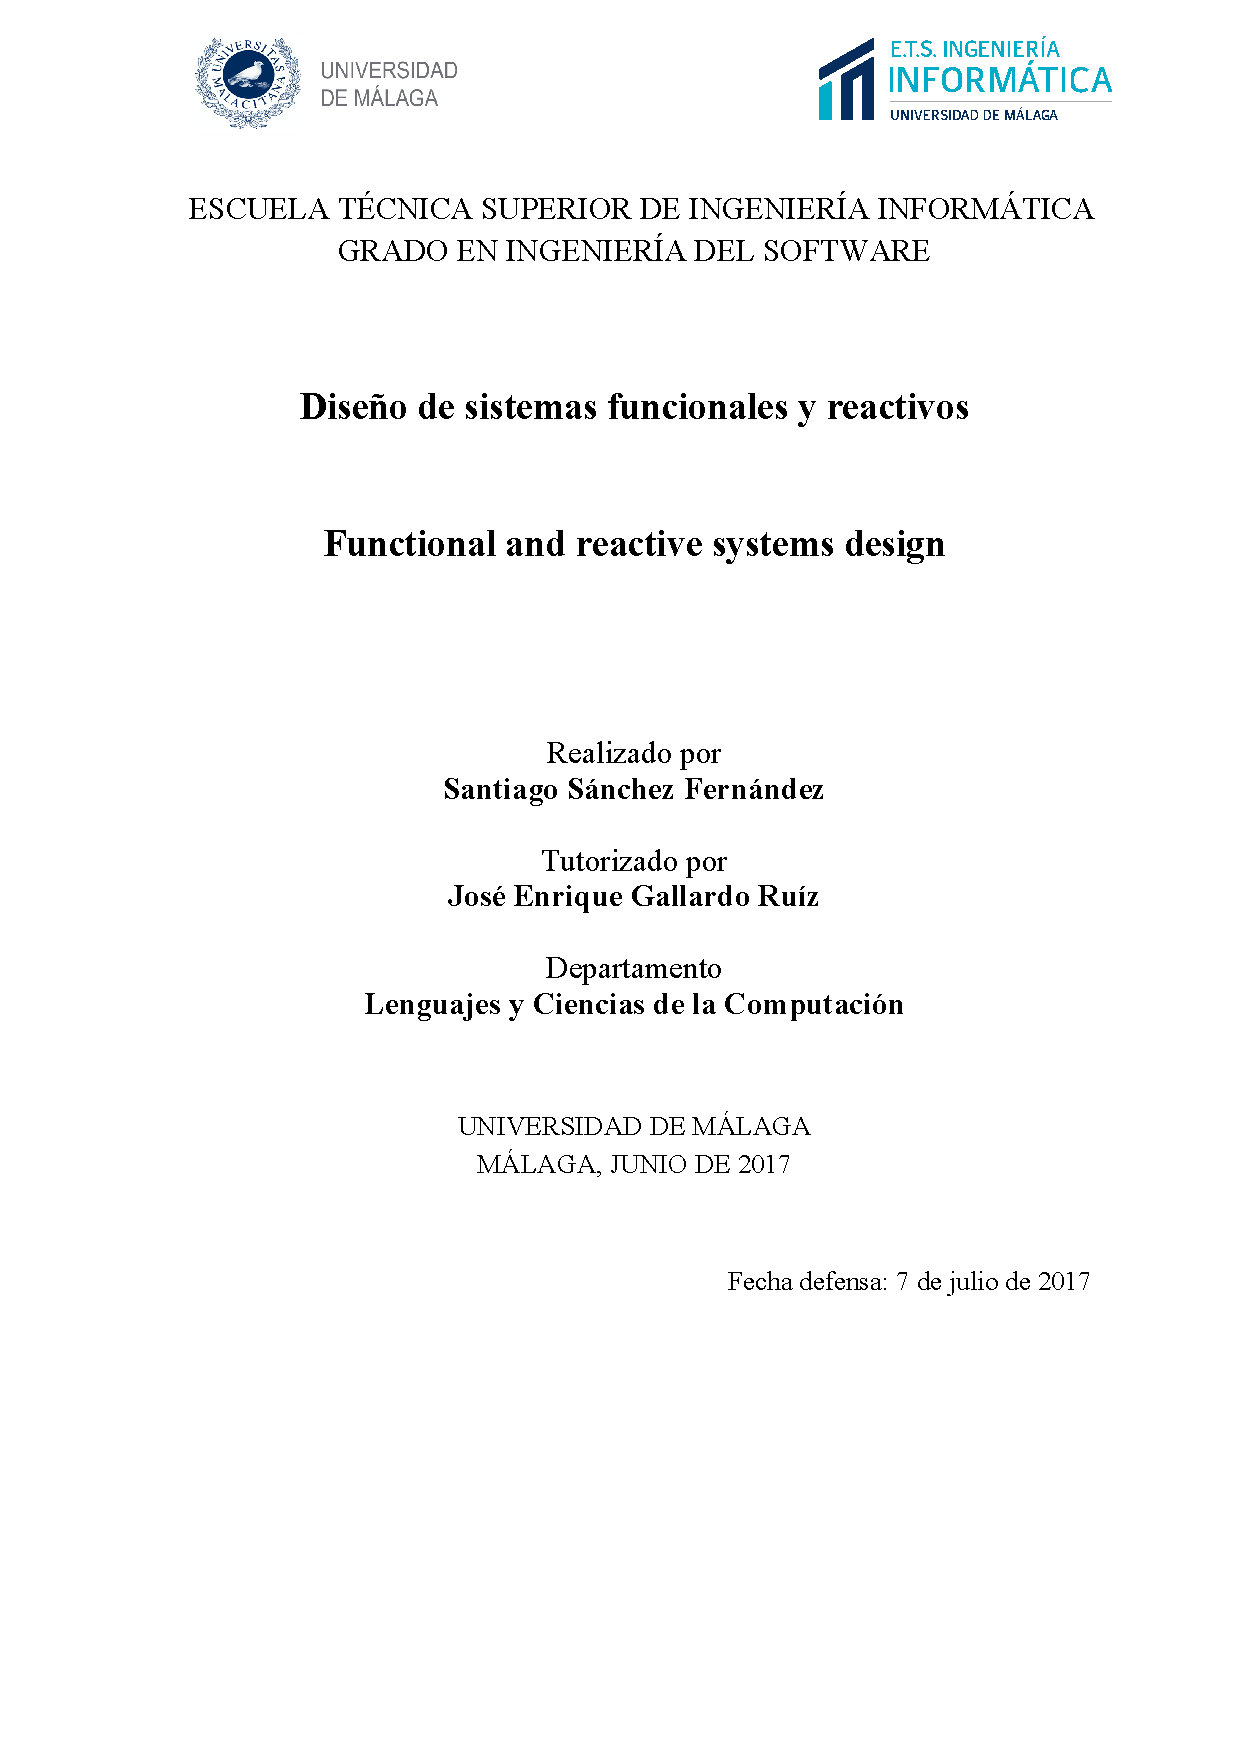
\includepdf[noautoscale=true, width=\paperwidth]{title.pdf}

\newpage

%% Abstract
\begin{abstract}

  \subsection{Español}
  Iot es una red de objetos físicos que están incrustados con electrónica, software, 
  sensores y conectividad de red, lo que permite a estos objetos recopilar y intercambiar datos.
  La IoT permite que los objetos sean detectados y controlados de forma remota a través de la 
  infraestructura de red existente, creando oportunidades para una integración más directa del mundo 
  físico en los sistemas basados en computadora, y resultando en una mayor eficiencia, precisión y 
  beneficio económico además de una reducción de la intervención humana.

  \subsection{English}
  IoT is a network of physical objects that are embedded with electronics, 
  software, sensors, and network connectivity, which enables these objects 
  to collect and exchange data. The IoT allows objects to be sensed and controlled 
  remotely across existing network infrastructure, creating opportunities for more 
  direct integration of the physical world into computer-based systems, and resulting 
  in improved efficiency, accuracy and economic benefit in addition to reduced human 
  intervention.

	\bfseries{\large{Keywords:}} IoT, FIWARE, Edificios Inteligentes
\end{abstract}

\tableofcontents

%% Sections
\section{Introducción}
\subsection{Motivación}
De acuerdo con (Estevez et al., 2021), la densidad de población que habita en las ciudades crece aceleradamente.
Se espera que para el 2030, un 60\% de las personas viva en las ciudades. 

Al existir una migración tan importante de áreas rurales a urbanas, el entorno de la
propia ciudad evoluciona más rápido y los retos a los que estas se enfrentan, o se espera que se enfrenten,
también cambian notablemente: el transporte, impacto medioambiental, salud pública, servicios, etc. Son puntos
críticos que merecen especial atención para mantener y mejorar el funcionamiento y la calidad de vida en
las urbes.

Todo esto, junto al crecimiento de las infraestructuras de telecomuncación (Banda ancha, wifi y 5G)
y a las inversiones en inteligencia artificial y big data, convierten  a Internet de las cosas (IoT)
 en un posible candidato para implementar soluciones y ofrecer mejoras a los gobiernos y ciudadanos, 
que ayuden a mejorar la gestión de las ciudades, la calidad de vida en las mismas y 
sean lo más respetuosas posible con el entorno.

Internet de las Cosas empezó siendo una sencilla idea de conectar dispositivos a
internet, la cual fue evolucionando de forma muy favorable y acabó evolucionando y 
mejorando en muchos aspectos. De hecho, según Elnashar, A. \& El-saidny, M. (2018),
en los últimos años, el uso del IoT ha aumentado, los presupuestos 
invertidos y el nº de dispositivos conectados han aumentado exponencialmente,

También es importante mencionar que la situación global de la COVID-19 ha incentivado
y acelerado la aplicación de la IoT en diversos aspectos como la salud pública,
la seguridad o la privacidad.

\subsection{Objetivos}
El objectivo principal va a consistir en desarrollar un sofware que, 
utilizando las tecnologías de IoT, aporte en el desarrollo tecnológico de las ciudades. 

Ya que uno de los pilares fundamentales de las ciudades son los edificios
que la componen, trabajar en un software para su gestión,
puede ser una buena aproximación para lograr este objetivo, por lo tanto, 
se va a buscar desarrollar un sistema que, usando IoT, permita gestionar
los edificios de una ciudad. Las funciones principales que se le van a pedir a 
este software van a ser, en rasgos generales, las siguientes:
\begin{itemize}
  \item Poder listar y filtrar los edificios que hay en una ciudad para tener información sobre ellos
        de una forma organizada.
  \item Conocer y gestionar la información de cada edificio indivialmente.
  \item Capacitar a los edificios de dispositivos IoT para mejorar la información que se puede ofrecer
        de estos y añadir interacciones para que realicen tareas como abrir la puerta o traer al 
        ascensor.
\end{itemize}
entre otros que se desarrollarán con más detalle en un documento de requisitos.

\subsection{Estructura del documento}
La estructura del documento va a estar orientada al análisis del proyecto que se va a
desarrollar. En una primera sección se va a hablar sobre un estudio previo de las tecnología 
 que se van a aplicar. Luego habrá una sección dedicada a la fase de captura de requisitos y organización
de tareas. A partir de ese momento, en el documento se explicarán y orgazarán cada una 
de las fases del proyecto.

\section{Estudio del arte}
En esta sección se va a realizar un análisis de las tecnologías que se van a emplear para el 
desarrollo del Software. Para ello, se va a comenzar con una revisión exahustiva de IoT: 
Qué es, qué podemos hacer con esta tecnología y qué problemas presenta que se deban de tener en cuenta.s
\subsection{Internet de las Cosas}
Internet de las Cosas es una red de objetos físicos que están incrustados con electrónica y poseen 
conectividad a la red, lo que permite a estos objetos recopilar e intercambiar datos.

Si bien el concepto de internet, que consiste en una red de usuarios y servidores conectados entre sí,
parece muy potente y ambiciosa, Internet de las cosas lo es más todavía, ya que además de abarcar a 
lo anterior, considera cualquier objeto físico como posible participante de la red.

Esto permite que los objetos sean detectados y controlados de forma remota a través de la  infraestructura de red existente, 
creando oportunidades para una integración más directa del mundo físico en los sistemas basados 
en computadora, y resultando en una mayor eficiencia, precisión y beneficio económico además 
de una reducción de la intervención humana. 

De esta forma podemos ser capaces de interactuar con los objetos de manera remota, sin intervención física de
una persona, o de manera automática.

Además, podrían realizar sus tareas de forma más inteligente, ya que, al estar conectadas a internet, pueden
disponer de mucha información útil para su objetivo.

Sumado a lo anterior, IoT es una tecnología relativamente reciente y son muchos los campos en los que 
todavía se puede aplicar para sacar ventaja. El potencial es muy elevado, y eso se puede ver en
conceptos como:
\begin{itemize}
  \item \textbf{IoT Orchestation}, que permite organizar los dispositivos para combinar sus operaciones
  y resultados, concediendo al sistema un mayor nivel de inteligencia.
  \item \textbf{Fog Computing}, que permite optimizar la comunicación entre dispositivos, evitando llamadas
  innecesarias a los servidores, mejorando la eficiencia y sostenibilidad.
  \item \textbf{Gemelo Digital}, que se trata de una representación digital, alimentada con información
  capturada con sensores y otros dispositivos digitales para que sea lo mas fiel posible, de un
  sistema real, del cual se hacen preguntas y se intenta gestionar.
  De esta forma se puede conocer el estado del sistema de una manera sencilla y se pueden simular supuestos
  (SandBbox) para observar qué ocurriría y en qué afectaria al sistema en general.
\end{itemize}
Todas esta características pueden aportar para una transformación digital inteligente y sostenible de las ciudades.

Entre de las ventajas más destacadas a la hora de usar IoT, podemos mencionar:
\begin{itemize}
    \item La sensorización: Permite obtener datos que anteriormente no podían ser recogidos de manera automática.
    \item Acciones remotas: Los objetos que se conectan a la red pueden realizar acciones físicas desencadenadas por internet,
      por lo que no tiene haber nadie presente ante el objeto para poder manipularlo o monitorizar su estado.
    \item Interacción entre dispositivos IoT: Gracias a los modelos de comunicación, se pueden realizar tareas complejas
      comunicando diferentes sensores y actuadores, de esta forma, se producen una secuencia de acciones sin necesidad
      de intervención humana, que produce unos resultados dignos de categorizar como inteligentes.
\end{itemize}


Por otro lado, al analizar el avance del IoT desde sus comienzos, se puede llegar a la conclusión 
de que ha ocurrido muy rápido, y todavía hay muchos puntos en los que debe de madurar:
\begin{itemize}
  \item Interfaces de Estandarización (Discovery, semántica de datos)
  \item Data Swamp (Discovery)
\end{itemize}

Por lo que a la hora de hacer un desarrollo usando IoT se deben de tener en cuenta estos aspectos.


\subsection{Plataforma FIWARE} 
Para el desarrollo de la plataforma, se ha decidido utilizar FIWARE.
Esta plataforma consiste en un ecosistema de componentes software basados en arquitectura
de código abierto que permiten la creación de aplicaciones basadas en la nube. Se utiliza 
principalmente para el desarrollo de aplicaciones en el ámbito inteligente, como es el de 
Internet de las cosas (IoT).

La visión de cómo construir los sistemas que plantea Fiware se basa en el paradigma de Gemelo Digital,
por lo tanto, a la hora de desarrollar la plataforma, hay que pregunstarse qué datos van a 
ser relevantes para el modelo que se quiere replicar. Por ejemplo, en un contexto de 
Buses inteligentes, puede resultar relevante datos como la localización del bus, 
el nº de pasajeros, quién es el conductor o cuál es la matricula del bus.

Uno de los puntos fuertes de Fiware radica en los diferentes niveles de obtención de datos.
Las plataformas más pequeñas recolectarán datos de sensores y sistemas de terceros,
pero una plataforma entera puede sevir como entrada de datos al Gemelo Digital, lo
cual hace más potente al sistema todavía.

\begin{figure}[h]
  \centering
  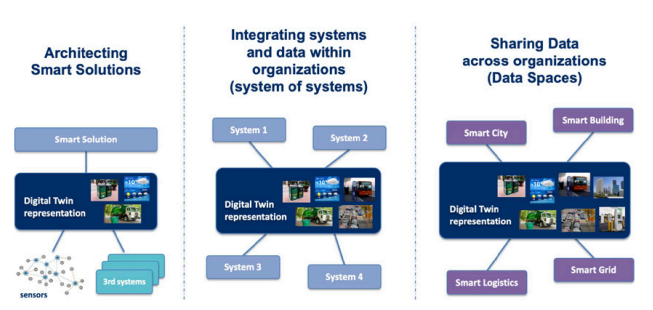
\includegraphics[width=0.8\textwidth]{digital_twin_levels_integration.png}
  \caption{Niveles de integración posibles siguiendo una aproximación con Gemelo Digital}
\end{figure}

Según el punto de vista de Fiware, las ciudades tienen 5 etapas en su camino a la digitalización inteligente:
\begin{itemize}
  \item Explotación vertical de Datos.
  \item Estandarización de modelos y APIs para la interoperabilidad de cualquier sistema.
  \item Datos abiertos (en tiempo real) para que terceros utilicen esos datos.
  \item Exportación del Sector privado de Datos. (Fiware incentiva con MarketPlace)
\end{itemize}

El elemento clave de integracion del ecosistema es el API NGSI 
(La última versión, NGSI-LD, que aprovecha el Linked Data para la 
interoperabilidad semántica). Entidades importantes como
la ETSI, GSMA, la Comisión Europea o el programa nacion de 
Smart City de India, apoyan y recomiedan el uso de esta interfaz como estándar.

Para que una plataforma se pueda calificar como "Basado en Fiware" debe de hacer uso
del Context Broker de Fiware que será el encargado de gestionar y facilitar los datos
de la plataforma. Alrededor de este Context Broker se encontrarán componentes que 
soportarán y facilitarán la captura, procesamiento, seguridad, etc. de los datos.

(Video conferencia de Canarias FIWARE)

\subsubsection{NGSI-LD}
NGSI-LD es una extension de JSON-LD. Eso significa que todos los NGSI-LD son JSON-LD,
pero no viceversa.

Como sabemos, JSON es un formato estándar de intercambio de datos, sin embargo, para
una máquina (incluso entre personas) puede ser dificil de interpretar el significado
de un dato que viene desde un JSON. Por ejemplo, un JSON con un campo name,
\begin{lstlisting}
  {"name": "alan turing"}
\end{lstlisting}
a priori no se sabe si name se trata del nombre de usuario de una plataforma o el 
nombre real de esa persona. Es por eso por lo que, aprovechando el concepto de
Linked Data, se desarrolló JSON-LD que se trata de una 
extensión de JSON incluyendo anotaciones sobre los datos (metainformación):
\begin{lstlisting}
{
  "@id": "https://uma.es/resources/informatica/tfg/2022/Alan_Turing",
  "@context": "https://json-ld.org/contexts/person.jsonld",
  "name": "alan turing"
}
\end{lstlisting}
Gracias al Linked Data, se definen los tipos de datos de forma estandar y tanto una 
persona como una máquina pueden tener un mejor entendimiento de qué significa cada dato
que viene en un JSON.

Los metadatos de JSON-LD vienen precedidos de un @, como en el ejemplo anterior:
@context es una URI que nos lleva a un diccionario que ayuda a interpretar los campos
del JSON asociando nombres a URIs donde se le otorga una definición
de manera estandar y @id es un URI del dato.

Con todo esto, podemos definir NGSI-LD, que no es más que la evolución de la versión
NGSI-V2, pero soportando el Linked Data. Sabiendo que NGSI-V2 es JSON, solo hacía
falta pasar a JSON-LD para implementar esa característica.

Para ello, se ha definido un @context por defecto denominado core NGSI-LD context
que se puede consultar desde la web de la etsi: https://uri.etsi.org/ngsi-ld/.
(No es necesario incluirlo en el @context)

Una de las cosas que hace es crear alias con los esquemas que más van a referenciar:
\begin{lstlisting}
"ngsi-ld": "https://uri.etsi.org/ngsi-ld/Date",
"geojson": "https://purl.org/geojson/vocab#"
\end{lstlisting}

También crean alias para los campos id y type, que ya se usaban en NSGI-V2,
dándole el significado que tienen @id y @type respectivamente en JSON-LD.

"id": "@id",
"type": "@type",

Otra diferencia fundamental es cómo se define el modelo de datos.
\begin{figure}[h]
  \centering
  \subfloat[NGSI-V2] {
    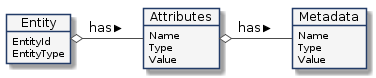
\includegraphics[width=0.3\textwidth]{ngsi-v2-model.png}
  }
  \subfloat[NGSI-LD] {
    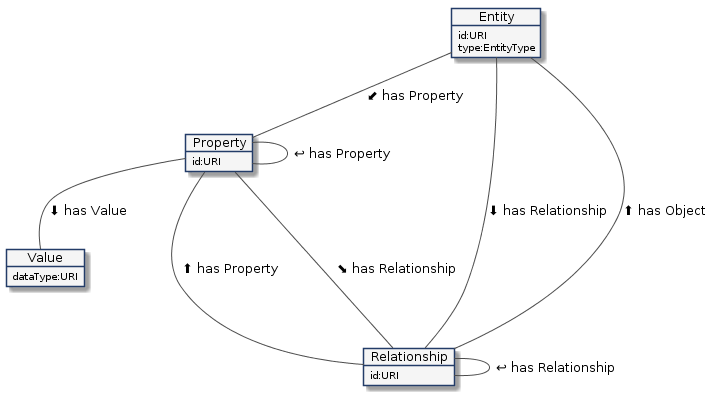
\includegraphics[width=0.4\textwidth]{ngsi-ld-model.png}
  }
  \caption{Modelo de datos NGSI}
\end{figure}

https://www.youtube.com/watch?v=rZ13IyLpAtA (Video Fiware Introducción NsGSI-LD)
https://fiware-datamodels.readthedocs.io/en/stable/ngsi-ld\_howto/index.html 
 (Documentación de Fiware sobre NGSI-LD)

\subsection{Ontología SAREF}
Se trata de una interfaz de datos que le gusta a la UE.

Gracias a ngsi-ld, podemos hace uso del modelo de datos.

\section{Metodología de trabajo}
Metodología de trabajo empleada en el TFG (esta parte también puede incluirse como una sección del capítulo de Introducción o como un capítulo independiente).
El proyecto va a seguir una metodología agile de tipo Scrum.


\section{Fases del proyecto}
Capítulos donde se estructure las fases del desarrollo, así como pruebas y resultados (si procede). 

En una primera fase se va a desarrollar un documento de requisitos donde aparecerán todos los detalles del producto.

En una segunda fase se van a desarrollar las tareas necesarias para el desarrollo del sistema y se van
a planificar en interaciones de sprint. 

\subsection{Captura de Requisitos}
En esta primera fase se va a hacer un estudio de lo que se quiere realizar, 
se van a analizar las diferentes tecnologías disponibles que se podrían usar y 
se van a plantear unos requisitos para, sobre ellos, organizar las tareas que 
se distribuirán en sprints para la realización del proyecto.

Los resultados de esta fase quedarán reflejados en un documento de requisitos, que 
utilizará como estructura la norma ISO: ISO/IEC/IEEE 29148:2018

\section{Conclusións e liñas de traballo futuras}
Conclusiones y Líneas Futuras. En caso de redactarse la memoria en inglés, las conclusiones y líneas futuras deben redactarse también en castellano.

\section{Contraportada}
%% Bibliography
\begin{thebibliography}{9}
\bibitem{Estevez}
Estevez E., Pardo, T., \& Scholl, J. (2021).
Smart cities and smart governance: towards the 22nd century sustainable city. Springer.
  \textit{The \LaTeX\ Companion}. 
  Addison-Wesley, Reading, Massachusetts, 1993.

\bibitem{Elnashar}
Elnashar, A. \& El-saidny, M. (2018). 
IoT evolution towards a super-connected world. Wiley.
  \textit{Practical Guide to LTE-A, VoLTE and IoT: Paving the way towards 5G}. pp. 310-381. 
  Wiley. https://doi.org/10.1002/9781119063407.ch7
  Ayman Elnashar; Mohamed A. El-saidny, "IoT Evolution Towards a Super‐connected World," in Practical Guide to LTE-A, VoLTE and IoT: Paving the way towards 5G , Wiley, 2018, pp.310-381, doi: 10.1002/9781119063407.ch7.

  
  \bibitem{einstein} 
  Albert Einstein. 
  \textit{Zur Elektrodynamik bewegter K{\"o}rper}. (German) 
  [\textit{On the electrodynamics of moving bodies}]. 
  Annalen der Physik, 322(10):891–921, 1905.

\end{thebibliography}

\newpage

%% Apendices
\begin{umaappendices}
\section{Installation \\ Manual}
Apéndices: información complementaria que no tenga cabida en el cuerpo del TFG, tales como listados, descripciones detalladas, manuales de usuario y programador, etc. 
  
  \textbf{\large{Requirements:}}
  
  \blindtext

\end{umaappendices}

\end{document}
